\documentclass{article}

\usepackage{graphicx}
\usepackage{tikz}
\usepackage{tikzsymbols}
\usetikzlibrary{calc,patterns,shapes.geometric}
\pagestyle{empty}
\usepackage[margin=0pt]{geometry}
\geometry{papersize={14in,12in}}

\def\centerarc[#1](#2)(#3:#4:#5){\draw[#1] ($(#2)+({#5*cos(#3)},{#5*sin(#3)})$) arc (#3:#4:#5);}

\begin{document}
	\begin{figure}
		\centering
		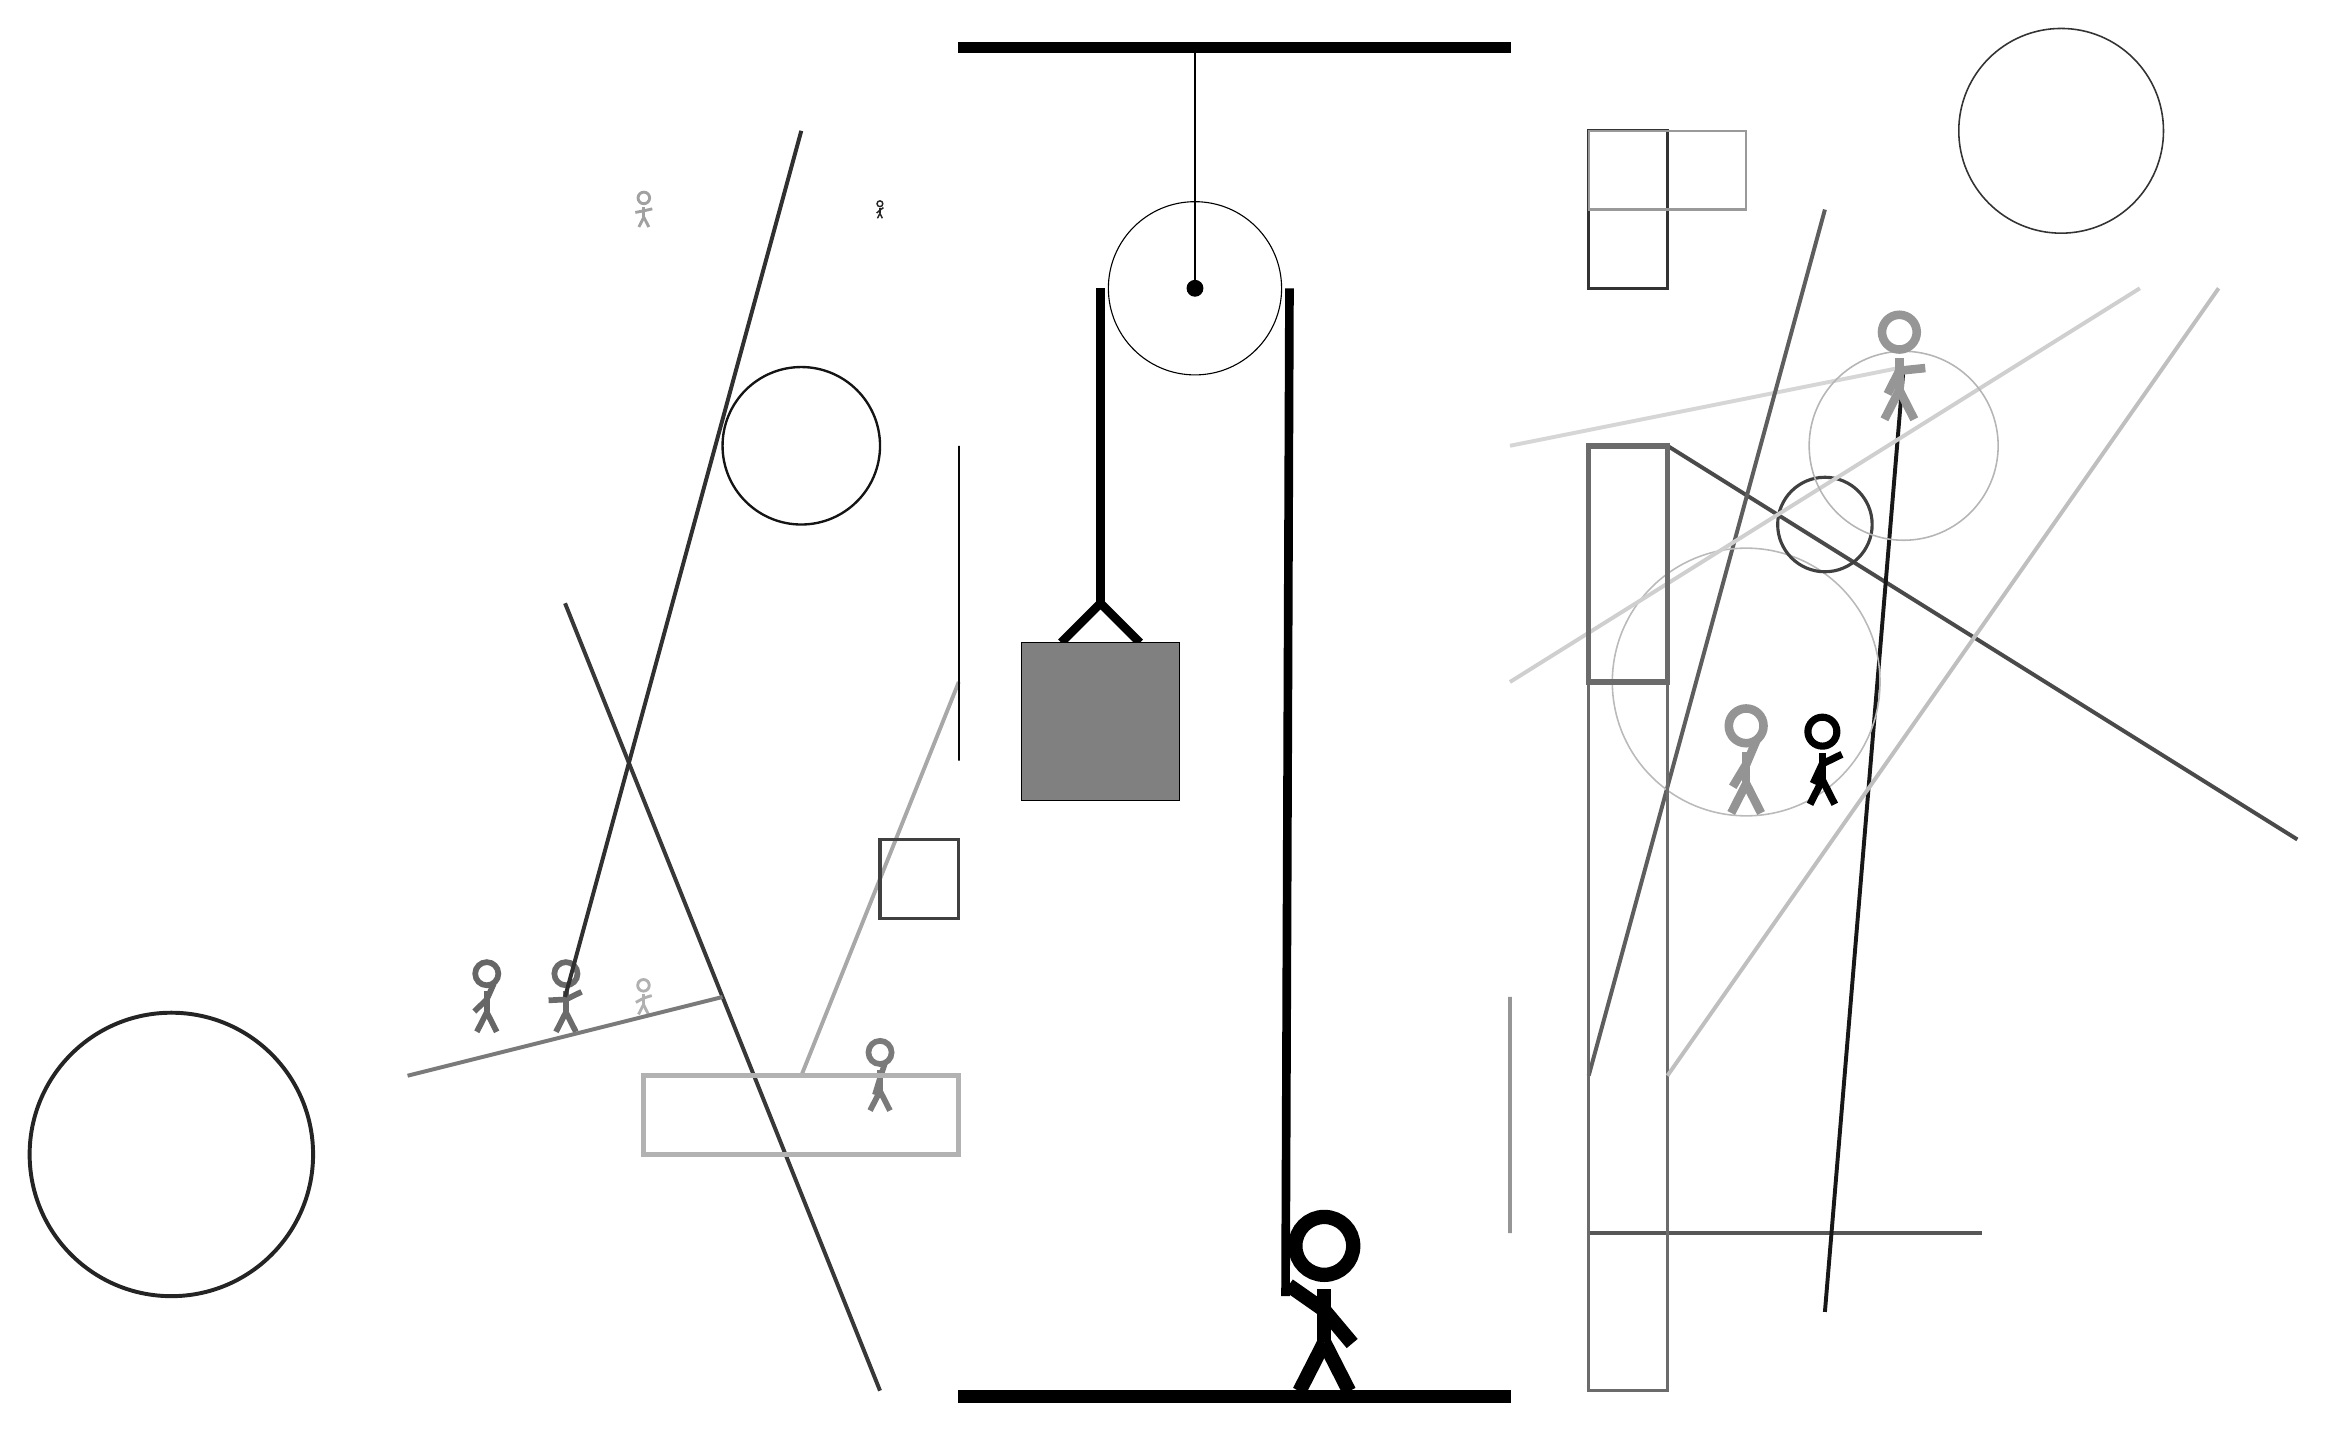
\begin{tikzpicture}
			%%%%% START %%%%%
			
			\draw[fill=black] (-2, 14) rectangle (5, 14.125);
			
			\draw (1, 11) circle (1.1);
			\draw[fill=black] (1, 11) circle (0.1);
			\draw (1, 14) -- (1, 11);
			
			\draw[line width=1.1mm] (-0.7, 6.5) -- (-0.2, 7.0) -- (0.3, 6.5);
			\draw[fill=black!50] (-1.2, 6.5) rectangle (0.8, 4.5);
			
			\draw[line width=1.1mm] (-0.2, 11) -- (-0.2, 7.0);
			\centerarc[line width=1.1mm](1, 11)(0:180:1.2000000000000002);
			\draw[line width=1.1mm](2.2, 11) -- (2.15, -1.8);
			
			\node at (2.6, -1.9) {\Strichmaxerl[10][-35][-50]};
			
			\draw[line width=0.5mm, color=black!71](7, 9) -- (15, 4);
			
			\draw[line width=0.5mm, color=black!34](-2, 6) -- (-4, 1);
			\draw[line width=0.5mm, color=black!16](5, 9) -- (10, 10);
			\draw[line width=0.5mm, color=black!41] (5, 2) rectangle (5, -1);
			
			\draw [line width=0.2mm, color=black!80](12, 13) circle (1.3);
			\node[line width=0.6mm, color=black!52] at (-3, 1) {\Strichmaxerl[4][73][72]};
			\draw[line width=0.5mm, color=black!66](6, -1) -- (11, -1);
			
			\node[line width=0.4mm, color=black!58] at (-7, 2) {\Strichmaxerl[4][3][26]};
			\draw[line width=0.5mm, color=black!91](9, -2) -- (10, 10);
			
			\node[line width=0.5mm, color=black!60] at (-8, 2) {\Strichmaxerl[4][44][66]};
			\draw[line width=0.5mm, color=black!78](-7, 7) -- (-3, -3);
			\draw[line width=0.5mm, color=black!63](9, 12) -- (6, 1);
			\draw [line width=0.5mm, color=black!86](-12, 0) circle (1.8);
			
			\draw [line width=0.2mm, color=black!27](8, 6) circle (1.7);
			\node[line width=0.3mm, color=black!86] at (-3, 12) {\Strichmaxerl[1][41][36]};
			\node[line width=0.3mm, color=black!31] at (-6, 2) {\Strichmaxerl[2][29][18]};
			
			\draw[line width=0.4mm, color=black!72] (-4, 6) rectangle (-4, 6);
			
			\draw[line width=0.5mm, color=black!52](-5, 2) -- (-9, 1);
			\draw [line width=0.3mm, color=black!92](-4, 9) circle (1.0);
			\draw [line width=0.4mm, color=black!75](9, 8) circle (0.6);
			\node[line width=0.4mm, color=black!100] at (9, 5) {\Strichmaxerl[5][65][26]};
			\draw[line width=0.5mm, color=black!19](5, 6) -- (13, 11);
			\node[line width=0.2mm, color=black!37] at (-6, 12) {\Strichmaxerl[2][11][13]};
			\draw[line width=0.4mm, color=black!80] (7, 11) rectangle (6, 13);
			\draw[line width=0.4mm, color=black!75] (-2, 4) rectangle (-3, 3);
			
			\node[line width=0.4mm, color=black!42] at (8, 5) {\Strichmaxerl[6][59][67]};
			\draw [line width=0.2mm, color=black!29](10, 9) circle (1.2);
			\draw[line width=0.7mm, color=black!58] (6, 6) rectangle (7, 9);
			\node[line width=0.2mm, color=black!41] at (10, 10) {\Strichmaxerl[6][63][6]};
			
			\draw[line width=0.2mm, color=black!97] (-2, 9) rectangle (-2, 5);
			\draw[line width=0.5mm, color=black!81](-7, 2) -- (-4, 13);
			\draw[line width=0.6mm, color=black!30] (-2, 1) rectangle (-6, 0);
			\draw[line width=0.4mm, color=black!58] (7, 9) rectangle (6, -3);
			
			\draw[line width=0.5mm, color=black!25](7, 1) -- (14, 11);
			
			\draw[line width=0.3mm, color=black!40] (6, 12) rectangle (8, 13);
			
			\draw[fill=black] (-2, -3) rectangle (5, -3.15);
			
			%%%%% END %%%%%
		\end{tikzpicture}
	\end{figure}	
\end{document}